\section[定位卫星]{定位卫星\\Satellite Position}
		本节以地球为中心在地心地固坐标系(ECEF)$X,Y,Z$中,通过开普勒轨道参数描述卫星的空间位置。选择开普勒参数的原因是,他们随着时间变化小。之后的五页研究这些轨道参数 $a,e,\omega,\Omega ,i,$ 和$\mu$,如图\ref{fig:9-7}。这是不可避免的技术;许多读者认为可以通过ECEF找到坐标,并继续。
	\begin{figure}
		\centering
		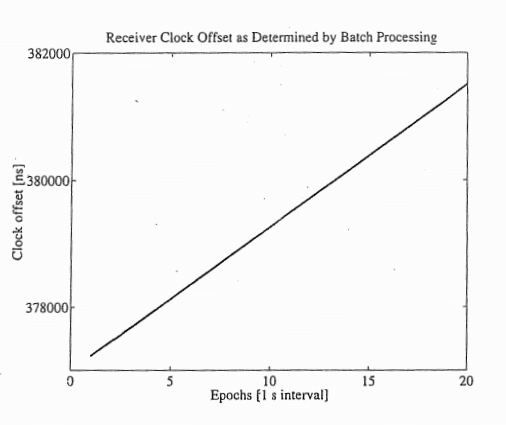
\includegraphics[width=0.7\linewidth]{TeX_files/Part03/chapter09/image/9-6}
		\caption{接收机时钟偏移量 $dt$}
		\label{fig:9-6}
	\end{figure}
	
	X轴指向赤道和格林威治子午线之间的交点。Z轴伴随着地球的自转轴。Y轴的指向正交于这两个方向,形成一个右手坐标系。
	
	轨道平面相交赤道平面交线。交线有两个点与赤道相交。卫星从南到北移动的经过的点称为升交点K。赤道平面和轨道平面之间的夹角称为轨道倾角i。地球中心C和X轴升交点K之间的夹角叫做$\Omega$;这是赤经。轨道上位置最接近地球中心的点(椭圆轨道的焦点)称为近地点。地球中心C、升交点K和近地点P之间的角叫做近地点角距$\omega$;这是从Z轴逆时针增加的方向观察的。
	\begin{figure}
		\centering
		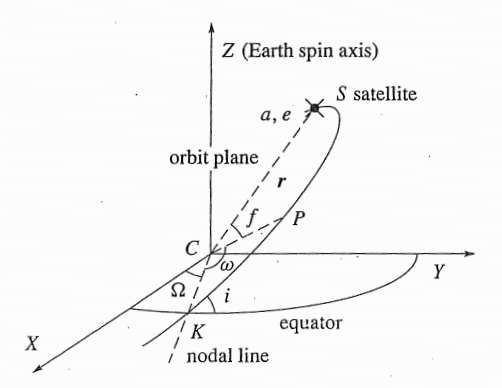
\includegraphics[width=0.7\linewidth]{TeX_files/Part03/chapter09/image/9-7}
		\caption{开普勒轨道参数:长半径 $a$,偏心率 $e$,轨道倾角 $i$,升交点$K$的赤经$\Omega$,近地点角距 $\omega$,和真近点角$f$. 近地点用$P$表示.。地球中心用$C$表示。}
		\label{fig:9-7}
	\end{figure}
	
	图\ref{fig:9-8}显示了轨道面在以地球为中心的坐标系平面中。$\xi$轴指向近地点$\eta$轴指向降交点。$\xi$轴和轨道面正交。从图\ref{fig:9-8}我们可以获得偏近点角$E$和真近点角$f$。我们可以获得:
	\begin{figure}
		\centering
		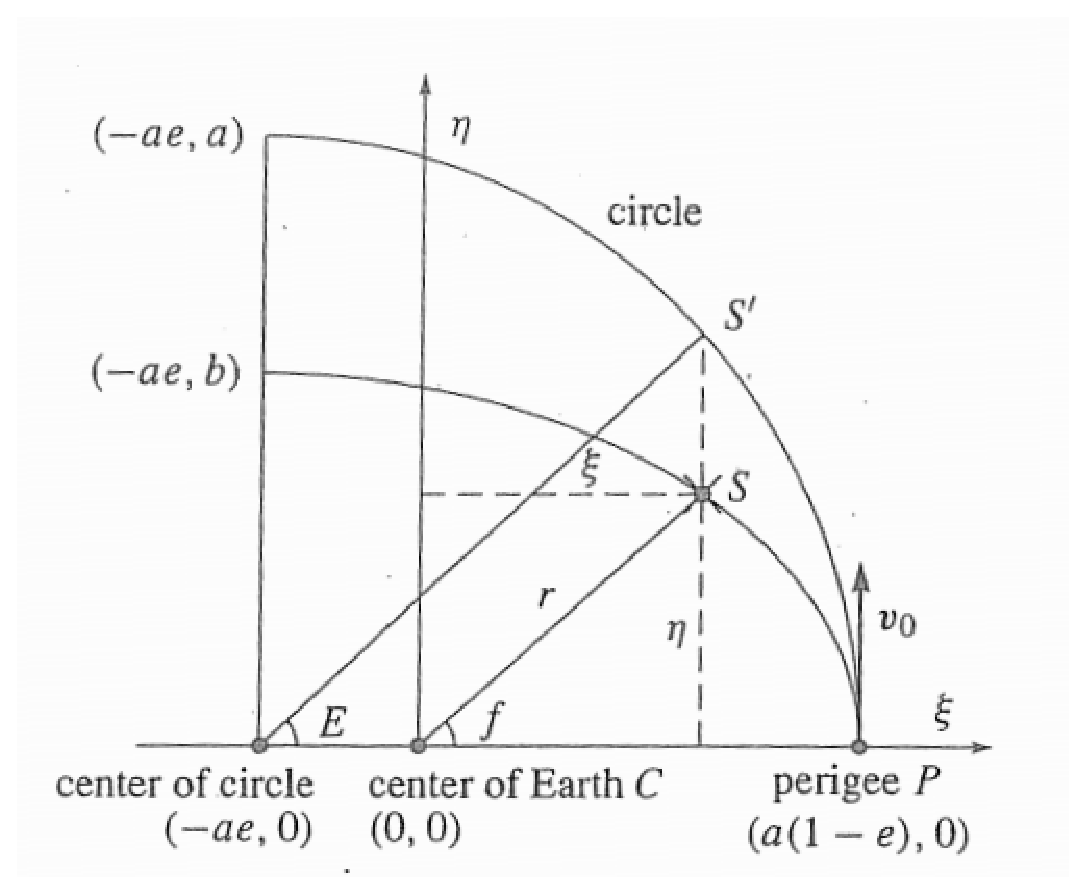
\includegraphics[width=0.7\linewidth]{TeX_files/Part03/chapter09/image/9-8}
		\caption{椭圆轨道在$(\xi,\eta)$坐标系中。真近点角$f$位于地球中心$C$.}
		\label{fig:9-8}
	\end{figure}
	$$\xi = r \cos f = a \cos E - ae = a (\cos E -e). $$
	$$\eta = r \sin f = \frac{b}{a} \sin E = b \sin E = a\sqrt{1-e^2}\sin E.$$
	
	因此,卫星坐标向量$r$在以地球中心$C$表示时是:
	\begin{equation}\label{eq:9.5}
	r=\begin{bmatrix}
	\xi \\ \eta \\ \zeta
	\end{bmatrix}
	=\begin{bmatrix}
	a(\cos E -e) \\
	a\sqrt{1-e^2}\sin E \\
	0
	\end{bmatrix}.
	\end{equation}
	
	通过三角函数变换可以得到下式:
	\begin{equation}\label{eq:9.6}
	\lVert r \lVert = a(1-e\cos E).
	\end{equation}
	一般角E随时间t变化,长半轴a和偏心率e几乎是恒定的。(对于e有长时间运行和短周期扰动,对于a只有短周期扰动。)$\lVert r \lVert$是卫星s到地球中心$C=(0,0,0)$的几何距离
	
	为了供以后参考我们引入平均值n即意味着角卫星运动速度。如果卫星的一个旋转周期是T,并且$GM = 3.986005 • 10^14 m^3/s^2$ 我们就有:	
	\begin{equation}\label{eq:9.7}
	n = \dfrac{2\pi}{T} = \sqrt{\dfrac{GM}{a^3}}.
	\end{equation}
	
	现在,是时候来定义平近点角$\mu$。这个非几何量定义为近地点和一个虚构的卫星之间的角度在圆形轨道卫星同样的焦距和同一周期的情况,但以一个恒定的速度移动。恒速是指卫星的运动。真实的和虚构的卫星穿越近地点和远地点的阶段,对于虚构的卫星,卫星的平均异常是真正的异常。是在t时刻的异常。(???)
	$$\mu = n(t-t_0)$$
	
	$t_0$是穿过近地点的时间。注意$\mu$ 是一个关于时间的线性函数的时间对于圆形轨道我们有$\mu = f + \omega$,参考Misra $\&$ Enge (2006).
	
	著名的开普勒方程关系两个角度,异常值$\mu$和偏近点角E:
	\begin{equation}\label{eq:9.8}
	E = \mu + e\sin E
	\end{equation}
	
	从式\ref{eq:9.5}中我们可获得
	\begin{equation}\label{eq:9.9}
	f = \arctan \frac{\eta}{\xi} = \arctan \dfrac{\sqrt{1-e^2}\sin E}{\cos E-e}
	\end{equation}
	这样我们获得了真近点角f,偏近点角E,平近点角$\mu$。这些关系式是计算卫星位置的基础。
	
	描述开普勒轨道六参数可以构成的一个轨道,所以他们在表\ref{tab:9.3}重复显示。
	
	重要的是要意识到轨道平面在地心坐标系X,Y,Z中仍相当稳定。换句话说:从太空轨道平面仍然和赤道保持固定关系。格林威治子午线平面绕地球自转轴的运动按照格林尼治恒星时(GAST),速度大约是24小时/天。GPS卫星每天绕行两周,它的轨道速度为3.87公里/秒。	
	
	卫星K的轨道平面在笛卡尔坐标系下的图像如图\ref{fig:9-7},我们可以获得
	$$\begin{bmatrix}
	r^k_j\cos f^k_j \\
	r^k_j\sin f^k_j \\
	0
	\end{bmatrix},$$
	
	$r^k_j = \lVert r(t_j)\lVert$由式\ref{eq:9.6}获得,其中$a,e,$和$E$是在时刻$t = t_j$时的值。
	
	这个向量旋转到X,Y,Z坐标系统的三维旋转矩阵对于图\ref{fig:9-7}为:
	$$R_3(-\Omega^k_j)R_1(-i^k_j)R_3(-\omega ^k_j).$$
	
	矩阵绕XY平面的旋转角为$\varphi$,同时Z方向不变。
	\begin{equation}\label{eq:9.10}
	R_3(\varphi) = 
	\begin{bmatrix}
	\cos \varphi & \sin \varphi & 0 \\
	-\sin \varphi & \cos \varphi & 0 \\
	0 & 0 & 1
	\end{bmatrix}
	\end{equation}
	
	同理$R_1(\varphi)$给出了关于X轴的旋转:
	
	\begin{table}
		\caption{卫星轨道的开普勒参数}
		\label{tab:9.3}
		\begin{tabularx}{\textwidth}{lX}
			\hline $a$ 长半轴 &  \multirow{2}*{轨道大小和形状参数} \\
			$e$ 偏心率 &  \\ 
			\hline $\omega$ 近地点角距 & \multirow{3}{150pt}{轨道平面的参数} \\ 
			$\Omega$ 升交点赤经 &  \\ 
			$i$ 倾角 &  \\ 
			\hline $\mu$ 平近点角 & 在平面的位置 \\ 
			\hline 
		\end{tabularx} 
	\end{table}
	
	\begin{equation}\label{eq:9.11}
	R_1(\varphi) = 
	\begin{bmatrix}
	1 & 0 & 0 \\
	0 & \cos \varphi & \sin \varphi \\
	0 & -\sin \varphi & \cos \varphi \\
	\end{bmatrix}
	\end{equation}
	
	卫星K在$t_j$时刻的地心坐标系下的坐标是:
	\begin{equation}\label{eq:9.12}
	\begin{bmatrix}
	X^k(t_j) \\ Y^k(t_j) \\ Z^k(t_j) 
	\end{bmatrix}
	=
	R_3(-\Omega ^k_j)R_1(-i^k_j)R_3(-\omega ^k_j)
	\begin{bmatrix}
	r^k_j \cos f^k_j \\
	r^k_j \sin f^k_j \\
	0
	\end{bmatrix}
	\end{equation}
	
	然而,GPS卫星不遵循了正常的轨道理论。我们必须使用与时间有关的更精确的轨道值:随时间变化的开普勒参数或与其等价的参数。在下文中,通过广播星历可以获得。我们把这些值插入在一个步骤后面,最后我们得到了一组变量式\ref{eq:9.12}。
	
	\begin{figure}
		\centering
		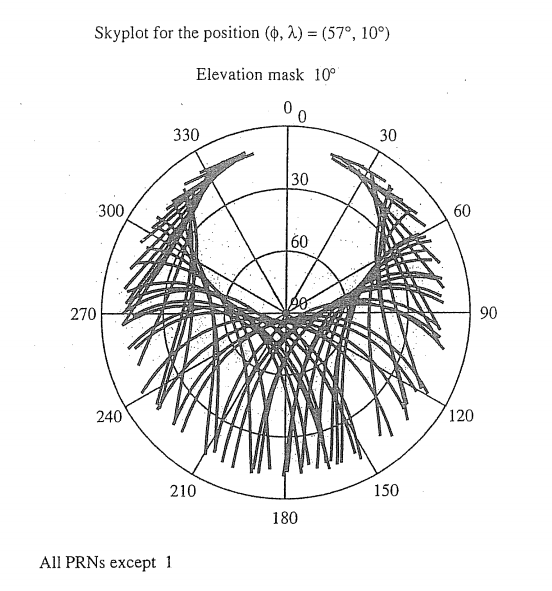
\includegraphics[width=0.7\linewidth]{TeX_files/Part03/chapter09/image/9-9}
		\caption{天空图包括所有GPS卫星在24小时内的给定位置。所有的高度角都为$10^\circ$。其中仅不包含1号卫星。}
		\label{fig:9-9}
	\end{figure}
	
	说一下卫星的星历表。这些参数值在一个特定的时间。每颗卫星传送其独特的星历数据。参数的描述实际的GPS卫星轨道及其开普勒轨道扰动参数。广播星历表使用之前直接计算轨道的一部分,和他们预测的下一个轨道的一部分。广播星历表是准确为1-2米。对于某些大地测量程序更好的精确性是必要的。一种可能性是获取精度在分米级的后处理精密星历表。
	
	星历表是用于从引用计数在GPS周秒时代t,它意味着间隔中心的星历是可用的。广播星历表的目的是在这段时间内使用。他们描述的是轨道2小时之后在指定位置的精度。他们预测4到6小时的曲线拟合数据。广播星历表包括
	
	$$\mu_0,\Delta n,e,\sqrt{a},\Omega_0,i_0,\omega,\dot{\Omega},\dot{i},C_{\omega c},C_{\omega s},C_{rs},C_{ic},C_{is},t_{oe}$$
	 
	在$\dot{\Omega}=\partial \Omega / \partial t$和$\dot{i}=\partial i / \partial t$。系数$C_\omega$,$C_r$,和$C_i$正确的近地点,轨道半径,由于不可避免的扰动理论和轨道倾角变化造成的轨道,地球的重力场,反射率和太阳的光压,太阳和月亮和潮汐力。星历表参数的参考时间是$t_{oe}$。
	
	考虑到传输时间t(在GPST时间)下面提供必要的变量供式\ref{eq:9.12}使用:
	\begin{table}
		\begin{tabularx}{\textwidth}{XX}
			\hline 过去的时间 $t_oe$  & $t_j=t-t_{oe}$ \\ 
			在$t_j$的平近点角 & $\mu_j = \mu_0 + (\sqrt{GM/a^3}+\Delta n)t_j$ \\ 
			地球的引力常数乘以质量 & $GM=3.986005\cdot 10^{14}M^3/S^2$ \\ 
			$E_j$的迭代解决方案  & $E_j=\mu_j+e\sin E_j$ \\ 
			真近点角  & $f_j=\arctan \dfrac{\sqrt{1-e^2}\sin E_j}{\cos E_j-e}$ \\ 
			升交点经度  & $\Omega_j=\Omega_0 + (\dot{\Omega_0}-\omega_e)t_j-\omega_et_{oe}$ \\ 
			地球平均自转   & $\omega_e=7.292115147\cdot10^{-5}rad/s$ \\ 
			近地点角距  & $\omega_j=\omega+f_j+C_{\omega c}\cos2(\omega+f_j)+C_{\omega s}\sin2(w+f_j)$ \\ 
			径向距离  & $r_j = a(1-e\cos E_j)+C_{rc}\cos 2(\omega+f_j)+C_{rs}\sin 2(\omega+f_j)$ \\ 
			轨道倾角  & $i_j = i_0+\dot{i}t_j+C_{ic}\cos 2(\omega+f_j)+C_{is}\sin 2(\omega+f_j)$ \\ 
			\hline 
		\end{tabularx} 
	\end{table}
	
	计算(9.12)的算法在M文件satpos中。函数计算GPS卫星的位置。它是每个位置计算的基础。为更多的细节在WGS84与GPS,见3.6节。
	
	这个m文件satposin计算卫星位置在一个惯性坐标系$\omega_e$ = 0中。
	
	关于开普勒元素的所有信息都包含在星历表。文件通过广播星历表时创建的GPS观测数据下载到一台笔记本电脑中。这些文件通常是特定的二进制格式。幸运的是可以转化为RINEX格式,这些格式见Gurtner(2000)。文件的后缀名第三个字符总是n(导航文件)。
	
	通常我们只需要导航信息中的一部分文件的星历文件。选择和重新格式化是通过以下命令:
	\begin{lstlisting}
	rinexe(ephemerisfile,outputfile);
	eph=get_eph(outputfile);
	satp=satpos(t,eph);
	\end{lstlisting}	
	\subsection[例子2]{例子2\\easy2}\label{subsec:easy2}
		第二个基本问题是计算以地球中心的惯性坐标系(ECI)中的给定位置的卫星伪距发出的时间。ECI GPS坐标系统使用地球赤道平面的方向是UTC时间2000年1月1日12时。x轴指向春分,z轴点北极的方向,y在是选为右手坐标系。
		\begin{figure}
			\centering
			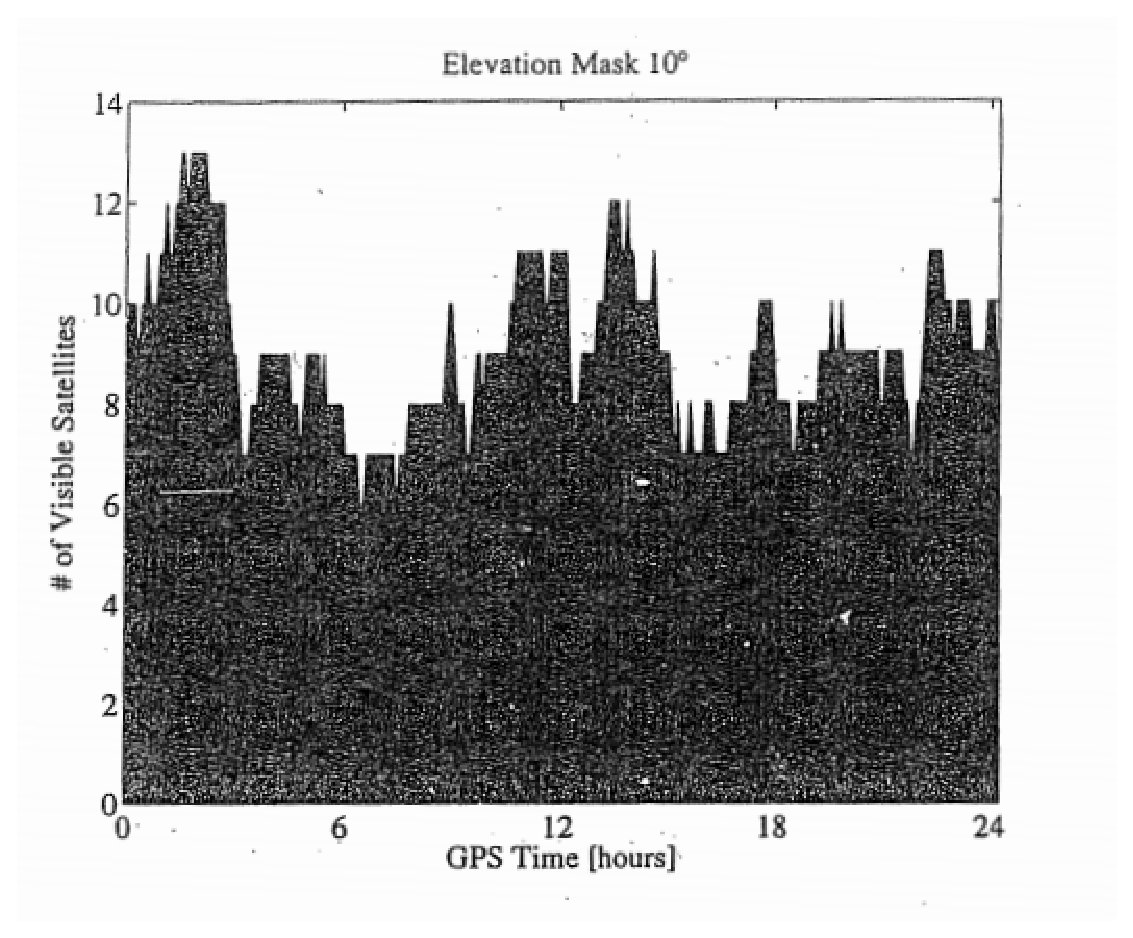
\includegraphics[width=0.7\linewidth]{TeX_files/Part03/chapter09/image/9-10}
			\caption{卫星高度角为$10^\circ$时}
			\label{fig:9-10}
		\end{figure}
		
		给定一个星历表从RINEX获得导航信息文件(n文件),easy2完成这个工作。主函数satpos实现GPS接口控制文档中描述的程序(IS-GPS-200 (2007)),表20-IV。
		
		我们读了RINEX格式的n文件,然后格式化成内部格式的MATLAB矩阵名叫Eph。此外,我们把Eph中的每一个卫星打印成一列。每一列包含21个变量;这些组成一个完整的卫星星历表一。
	
	\subsection[例子11]{例子11\\easy11}\label{subsec:easy11}
		图\ref{fig:9-9}展示了卫星轨道的极坐标图在一个地球上给定的位置。你可以看到的时间连续24小时期间每个卫星都是可见的。
		\begin{figure}
			\centering
			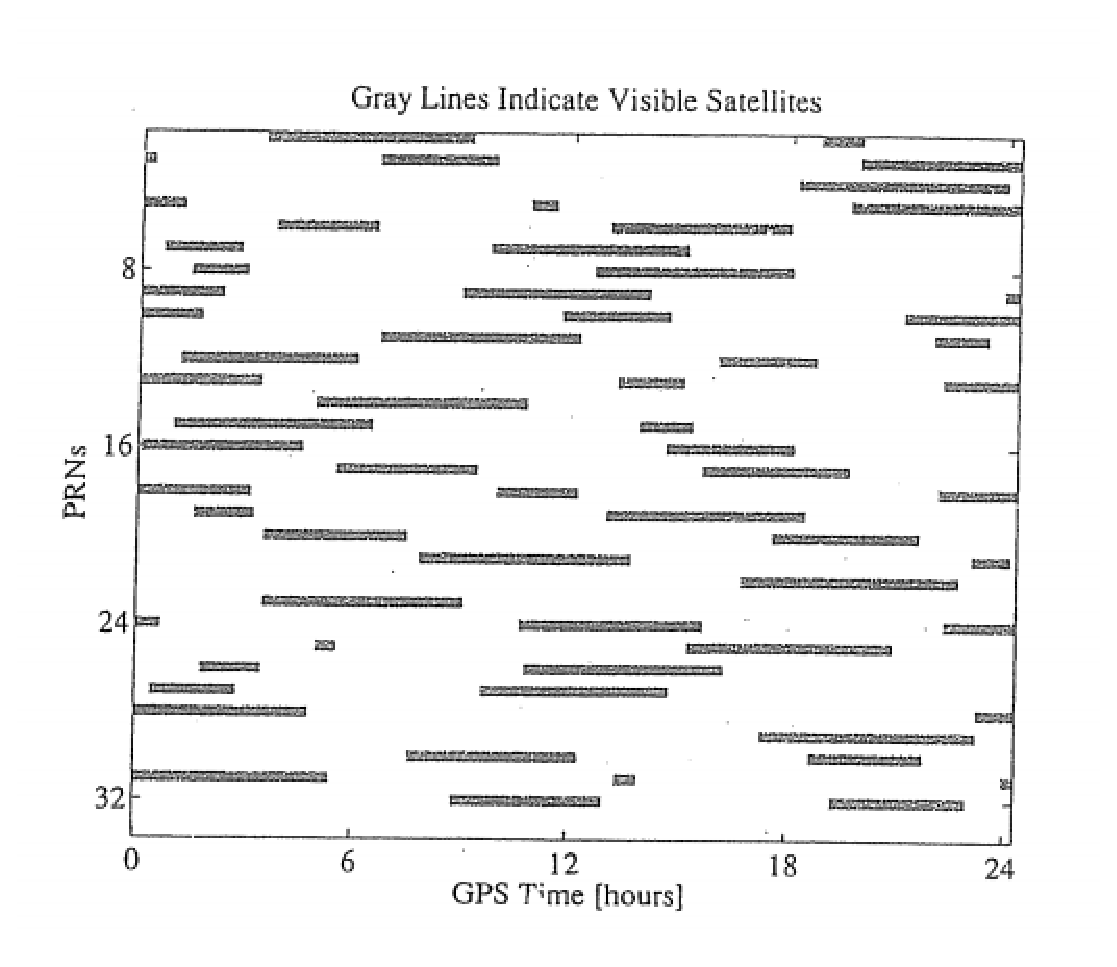
\includegraphics[width=0.7\linewidth]{TeX_files/Part03/chapter09/image/9-11}
			\caption{高度角大于等于$10^\circ$在 $\varphi = 57^\circ$和$\lambda = 10^\circ$位置的卫星}
			\label{fig:9-11}
		\end{figure}
		
		easy11是基于历书下载的最方便的国家大地测量服务ngs.noaa.gov/CORS/Data.html。实际的文件名是brdcl550.08n。
		
		MATLAB的RINEX文件已被重新格式化为二进制格式的卫星星历表,以提供给M文件rinexe使用。用户输入$(\varphi,\lambda)$的位置可以看到在这点的图像和一个需要设置的海拔值,然后将绘制所有可见的方位角和高度角的位置以及卫星计算和绘制极坐标。
		
		下一个遵循记录有多少,哪些卫星可见白天时间当他们可以看到。 图\ref{fig:9-10}和\ref{fig:9-11}将显示这些点。
		
		MATLAB代码很简单,结果令人印象深刻,它是有用的。在早期GPS星座是不完整的。这样的程序尤其有价值,为达成计划的目的是确保足够的卫星可以定位。除了最严重的地形和城市峡谷,接收器可以找到大量的GPS和GLONASS卫星,这种情况会在伽利略卫星发射后变得更加令人满意。
	
